\documentclass[9pt,twocolumn,twoside]{styles/osajnl}
\usepackage{fancyvrb}
\usepackage{graphicx}
\journal{i524} 

\title{An overview of HadoopDB and its Architecture}

\author[1]{Karthik Anbazhagan}

\affil[1]{School of Informatics and Computing, Bloomington, IN 47408, U.S.A.}

\affil[*]{Corresponding authors: kartanba@iu.edu}

\dates{\today}

\ociscodes{Cloud, MapReduce, I524}

% replace this with your url in github/gitlab
\doi{\url{https://github.com/kartanba/sp17-i524/blob/master/paper1/S17-IR-2008/report.pdf}}


\begin{abstract}
With an explosion in data available for analysis, database management for the analytical applications is rapidly changing from high-end proprietary machines towards a cheaper, lower-end hardware, and virtual environment inside clouds. This paper speculates the feasibility of using a cost efficient system that is a hybrid between a parallel database and a MapReduce-based system that takes the best features of both systems.
\newline
\end{abstract}

\setboolean{displaycopyright}{true}

\begin{document}

\maketitle 


\section{Introduction}
The proliferation of sensors and data capturing devices, coupled with the evolution and the increase in automation process has resulted in the capture and storage of data. The amount of data that is stored and processed by analytical database systems are growing at an immense rate. More and more historical data are being accumulated and kept online for future analysis. With the data explosion problem, companies are forced to upgrade themselves to a cheaper yet more efficient database management system. Since the data analysis workloads consist of many large-scale operations, complex aggregations, and star schema joins, parallelization of databases across nodes in a cluster and usage of a MapReduce system is increasingly getting more attention. MapReduce or its available alternate as open source Hadoop processes structured data, and can do so at tremendous scale. Hadoop is being used to manage Facebook’s 2.5 petabyte data warehouse. 

HadoopDB\cite{hadoopdb} is and open source component that serves as exactly such a hybrid system. It is a hybrid of a parallel database and MapReduce technologies. It approaches parallel databases in performance and efficiency, and also yields the scalability, fault tolerance, and flexibility of MapReduce systems. It uses PostgreSQL as the database layer and Hadoop as the communication layer, Hive as the translation layer. It has been demonstrated on clusters with 100 nodes and should scale as long as Hadoop scales. 

\section{Components of HadoopDB}
A HadoopDB \cite{hadoopdb-project} system consists of two main components whose best of features it tries to adapt and provide a hybrid system of the two. This section describes in brief about the components and describes the best features and the shortfalls of the two main components of HadoopDB.

\subsection{Parallel DBMSs}
The parallel DBMS are the most recent systems that are support standard relational tables and SQL. In this DBMS the data partition is transparent to the end-user. Parallel databases use an optimizer tailored for distributed workloads into a query plan whose execution is divided equally among multiple nodes.
 
Parallel databases can achieve especially high performance when administered by someone who can carefully design, deploy, tune, and maintain the system. It also has a very flexible query interface property which contains an implementation of SQL and ODBC which are an important part of the analytical data management picture. Parallel databases however generally do not score well on the fault tolerance and ability to operate in a heterogeneous environment properties. 
    
\subsection{MapReduce systems}
MapReduce system processes data distributed (and replicated) across many nodes in a shared-nothing cluster via three basic operations. First, a set of Map tasks are processed in parallel by each node in the cluster without communicating with other nodes. Next, data is repartitioned across all nodes of the cluster. Finally, a set of Reduce tasks are executed in parallel by each node on the partition it receives. Unlike parallel database, MapReduce does not create a detailed query execution plan. It is determined at runtime. This allows MapReduce to assign more tasks to faster nodes and reassigning tasks from failed nodes. 

One of the biggest issue with MapReduce is performance. By not requiring the user to first model and load data before processing, many of the performance enhancing tools used by database systems are not possible. MapReduce has a flexible query interface; Map and Reduce functions are just arbitrary computations written in a general-purpose language. It best meets the fault tolerance and ability to operate in heterogeneous environment properties. It achieves fault tolerance by detecting and reassigning Map tasks of failed nodes to other
nodes in the cluster.

\begin{figure}[h]
    \centering
    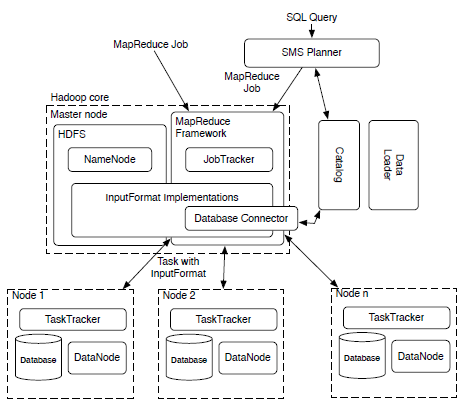
\includegraphics[width=8cm]{images/hadoopDB.png}
    \caption{Architecture of HadoopDB system}
\end{figure}

\section{Architecture}

Fig 1. shows the architecture\cite{hadoop-guide} of a model for using the HadoopDB system. It is very essential to understand every component of the architecture to understand how hadoopDB works. This section describes in brief about the components that are part of the hadoopDB architecture.

As shown in Figure 1., HadoopDB connects to multiple single node database systems using Hadoop as the task coordinator and network communication layer. Queries are parallelized across nodes using the MapReduce framework. HadoopDB achieves fault tolerance and the ability to operate in heterogeneous environments by
inheriting the scheduling and job tracking implementation from Hadoop.

\subsection{HadoopDB Layers}
At the heart of HadoopDB is the Hadoop\cite{apache-hadoop} framework. Hadoop consists of two layers: \\(i) a data storage layer or the Hadoop \cite{apace-web-page} Distributed
File System (HDFS) \\(ii) a data processing layer or the MapReduce Framework.

HDFS\cite{hadoop-cluster-setup} is a block-structured file system managed by a central NameNode. Individual files are broken into blocks of a fixed size and distributed across multiple DataNodes in the cluster. The
NameNode maintains metadata about the size and location of blocks and their replicas.
The MapReduce Framework follows a simple master-slave architecture. The master is a single JobTracker and the slaves or worker nodes are TaskTrackers. The JobTracker handles the runtime
scheduling of MapReduce jobs and maintains information on each TaskTracker’s load and available resources. Each job is broken down into Map tasks based on the number of data blocks that
require processing, and Reduce tasks. The JobTracker assigns tasks to TaskTrackers based on locality and load balancing. It load-balances by ensuring all available TaskTrackers are assigned tasks. TaskTrackers regularly update the JobTracker with their status through heartbeat messages.


\subsection{Other Components of HadoopDB}

\subsubsection{Database Connector}
The Database Connector is the interface between independent database systems within the nodes in the multinode cluster and TaskTrackers. Each MapReduce job supplies the Connector with an SQL query and connection parameters such as which JDBC driver to use, query fetch size and other query tuning parameters. The Connector connects to the database, executes the SQL query and returns results as key-value pairs.

\subsubsection{Catalog}
The catalog maintains information about the databases:
\\(i) connection parameters such as database
location, driver class and credentials, 
\\(ii) metadata such as data sets contained in the cluster, replica locations, and data partitioning properties.

The current implementation of the HadoopDB catalog stores its information as an XML file in HDFS. This file is accessed by the JobTracker and TaskTrackers to retrieve information necessary
to schedule tasks and process data needed by a query.

\subsubsection{Data Loader}
The Data Loader is responsible for 
\\(i) globally repartitioning data on a given partition key upon loading, 
\\(ii) breaking apart single node data into multiple smaller partitions or chunks and 
\\(iii) finally bulk-loading the single-node databases with the chunks.

The Data Loader consists of two main components: Global Hasher and Local Hasher. The Global Hasher executes a custom made MapReduce job over Hadoop that reads in raw data files stored in HDFS and repartitions them into as many parts as the
number of nodes in the cluster. The Local Hasher then copies a partition from HDFS into the
local file system of each node and secondarily partitions the file into smaller sized chunks based on the maximum chunk size setting.

\subsubsection{SQL to MapReduce to SQL (SMS) Planner}
HadoopDB provides a parallel database front-end to data analysts enabling them to process SQL queries. The SMS planner extends Hive\cite{facebook-hive} which transforms HiveQL, a variant of SQL, into MapReduce jobs that connect to tables stored
as files in HDFS. The MapReduce jobs consist of DAGs of relational operators such as filter, select, join, aggregation that operates as iterators. Since each table is stored as a
separate file in HDFS, Hive assumes no collocation of tables on nodes.


\section{CONCLUSION}

This paper has given an overview and the architecture of HadoopDB which give a clear picture of the hybrid system. We see that HadoopDB does not replace Hadoop. Both systems coexist enabling the analyst to choose the appropriate tools for a given dataset and task.  We also find that HadoopDB can approach the performance of parallel database systems while achieving similar scores on fault tolerance, an ability to operate in heterogeneous environments, and software license cost as Hadoop. 

HadoopDB is, therefore, a hybrid of the parallel DBMS and Hadoop approaches to data analysis, achieving the performance and efficiency of parallel databases, yet still yielding the scalability, fault tolerance, and flexibility of MapReduce-based systems. The ability of HadoopDB to directly incorporate Hadoop and open source DBMS software makes HadoopDB particularly flexible and extensible for performing data
analysis at the large scales expected of future workloads.

\bibliography{references.bib}

\end{document}
